% main.tex
\documentclass[12pt]{scrreprt}
\usepackage[a4paper, margin=2.5cm]{geometry}
\usepackage{xcolor}
\usepackage{listings}
\usepackage{underscore}
\usepackage[english]{babel}
\usepackage{scrlayer-scrpage}
\usepackage{setspace}
\usepackage{titlesec}
\usepackage[utf8]{inputenc}
\usepackage{placeins}
\usepackage{float}
\usepackage{graphicx}
\usepackage{caption}    % 允许子图使用 caption
\usepackage{subcaption} 
\usepackage{array}
\usepackage{colortbl}
\usepackage{booktabs}
\usepackage[bookmarks=true]{hyperref}
\usepackage{parskip}           % 段落间距
\setlength{\parskip}{0.5em}    % 紧凑段落间距
\renewcommand{\baselinestretch}{1.05} % 行距微调

% main.tex导言区
\usepackage{titlesec}
\titleformat{\chapter}[block]
{\normalfont\huge\bfseries}{\thechapter}{1em}{}
\titleformat{\section}[block]
{\normalfont\Large\bfseries}{\thesection}{1em}{}
\titleformat{\subsection}[block]
{\normalfont\large\bfseries}{\thesubsection}{1em}{}
% 保持编号与标题的经典间距
\makeatletter
\renewcommand{\@seccntformat}[1]{\csname the#1\endcsname\quad}
\makeatother

% 现代间距系统(单位:pt)
\titlespacing*{\chapter}{0pt}{25pt}{15pt}  % 上间距25pt/下间距15pt
\titlespacing*{\section}{0pt}{15pt}{7pt}
\titlespacing*{\subsection}{0pt}{10pt}{5pt}

% 确保子章节编号
\setcounter{secnumdepth}{3}
\setcounter{tocdepth}{3} % 目录显示到三级标题

% 封面字体优化
\usepackage{anyfontsize}        % 精确字体控制
\usepackage[sfdefault]{noto}   % 现代无衬线字体(需要安装Noto Sans字体)

%refers
\usepackage[style=ieee, sorting=none, backend=biber]{biblatex}
\addbibresource{re.bib}

% Hyperref配置
\hypersetup{
    pdftitle={Software Requirement Specification},
    pdfauthor={Jean-Philippe Eisenbarth},
    pdfsubject={TeX and LaTeX},
    pdfkeywords={TeX, LaTeX, SRS, Requirements},
    colorlinks=true,
    linkcolor=blue!70!black,
    citecolor=green!60!black,
    filecolor=magenta,
    urlcolor=cyan!70!black,
    linktoc=page
}

% 全局格式设置
\setstretch{1.1}
\titleformat{\chapter}[display]
{\normalfont\huge\bfseries}{\chaptertitlename\ \thechapter}{20pt}{\Huge}
\titlespacing*{\chapter}{0pt}{-30pt}{40pt}

% 自定义命令
\newcommand{\placeholder}[1]{\textcolor{gray!70}{\textlangle\,\textit{#1}\,\textrangle}}
\newcommand{\req}[2]{\item[REQ-#1:] #2} %详见设置文件

\newcommand{\myversion}{1.4}   %在这里更改文档版本

\begin{document}

% 封面
% cover.tex
\begin{flushright}
    \vspace*{1.5cm}
    \rule{0.75\textwidth}{5pt}
    
    \vspace{1.2cm}
    \fontsize{30}{28}\selectfont
    \textbf{Detailed Design}
    
    \vspace{1.5cm}
    \fontsize{14}{16}\selectfont
    for
    
    \vspace{1cm}
    \fontsize{18}{22}\selectfont
    Design and Implementation of a Lightweight \\[0.3em]
    Education Data Bay Area (E-DBA)
    
    \vspace{1.5cm}
    \fontsize{13}{15}\selectfont
    Version \myversion\ Approved
    
    \vspace{1.8cm}
    \begin{minipage}{0.7\textwidth}
    \flushright
    \fontsize{12}{14}\selectfont
    \textbf{Prepared by:} \\
    Taian Yu (FULL)\quad Yolanda Yin (FULL) \\
    Justin Zhang (FULL)\quad Aaron Liu (FULL) \\
    Steven Luo (FULL)\quad Younger Yang (FULL)
    \end{minipage}
    
    \vspace{1.2cm}
    \fontsize{14}{16}\selectfont
    Group C01
    
    \vspace{2cm}
    \today
\end{flushright}

% 目录
\tableofcontents

%迭代历史
\chapter*{Revision History}
\begin{center}
    \rowcolors{2}{gray!15}{white} % 设置表格隔行颜色
    \begin{tabular}{>{\raggedright\arraybackslash}p{3.5cm}
                    >{\raggedright\arraybackslash}p{3cm}
                    >{\raggedright\arraybackslash}p{5cm}
                    >{\centering\arraybackslash}p{2cm}}
        \toprule[1.5pt]
        \rowcolor{gray!30} % 表头颜色
        \textbf{Name} & \textbf{Date} & \textbf{Reason For Changes} & \textbf{Version}\\
        \midrule
        All Members & 9 April & Create the document & 1.0\\
        \bottomrule[1.5pt]
    \end{tabular}
\end{center}



\chapter{Introduction}

All external database interfaces mentioned in the document (such as the student information database, the degree thesis database, the bank account database, etc.) should be integrated and invoked according to the interfaces configured by the providers.

\section{Purpose}
This Software Requirements Specification (SRS) document defines the functional, performance, and system constraints for the Educational Data Platform (E-DBA). It serves as a comprehensive reference for developers, testers, project managers, and other stakeholders to ensure a shared understanding of the system's expected behavior and requirements. This document will act as the foundation for system design, development, testing, and validation while ensuring that the implementation aligns with the specified business and technical needs.

\section{Document Conventions}
This document adheres to the following standardized conventions:

\subsection{Formatting and Typography}
The documentation maintains consistent typographic practices, with body text in a uniform font and size. Headings are bolded and organized in a hierarchical structure through section divisions to clarify content organization.

\subsection{Terminology Guidelines}
Key terms are consistently defined and formatted for clarity. For example, \textbf{data providers} and \textbf{data consumers} refer to user roles that supply data to the system and retrieve data from the system, respectively.

\subsection{Modular Structure}
Content is structured according to the system’s functional components and modules, such as user role management, data-sharing services, payment systems, and other operational divisions, ensuring logical separation and ease of navigation.

\section{Intended Audience and Reading Suggestions}

This document is intended for the following audience groups:

\begin{itemize}
    \item \textbf{Project Managers and Developers:}  
    Should begin with the overview section to understand the system’s architecture and objectives, followed by the functional and technical requirements sections to gain insights into implementation details.  
    \item \textbf{System Administrators:}  
    Recommended to focus on the system configuration and management sections, including administrator privileges, security settings, and maintenance workflows.  
    \item \textbf{End Users (e.g., students, faculty, and staff):}  
    Advised to refer directly to the user guide and role-specific tutorials to learn how to access and utilize the E-DBA platform’s services effectively.  
\end{itemize}

By following these reading paths, each audience group can efficiently locate relevant information aligned with their roles and responsibilities.

\section{Project Scope}
The development of the E-DBA platform’s user interface, backend management system, and associated service modules, alongside the implementation of role-based access control for diverse user categories such as administrators, organizational coordinators, and data providers. Core functionalities include data provisioning and consumption mechanisms covering student identity verification, degree thesis access, and course information sharing, as well as the integration of a multi-payment-method online transaction system. Additionally, the platform will offer data warehousing capabilities to enable dataset export and collaborative sharing. Emphasis is placed on ensuring cross-institutional compatibility, robust data security protocols, and intuitive user experience design to streamline data interoperability and service delivery across participating educational organizations.

\section{References}
Foundational insights are drawn from the Eclipse Dataspace Connector (EDC) framework documentation, including its technical specifications and implementation guidelines for secure data exchange. Architectural principles align with the reference models and interoperability standards published by the International Data Spaces Association (IDSA). Additionally, compliance considerations incorporate relevant educational data governance frameworks, cross-institutional data-sharing policies, and sector-specific regulatory requirements. Technical implementation details are informed by industry-standard development protocols, API integration best practices, and security benchmarks for distributed systems, ensuring alignment with modern data infrastructure paradigms.


\chapter{Overall Description}

\section{Product Perspective}
\begin{figure}[h]
    \centering
    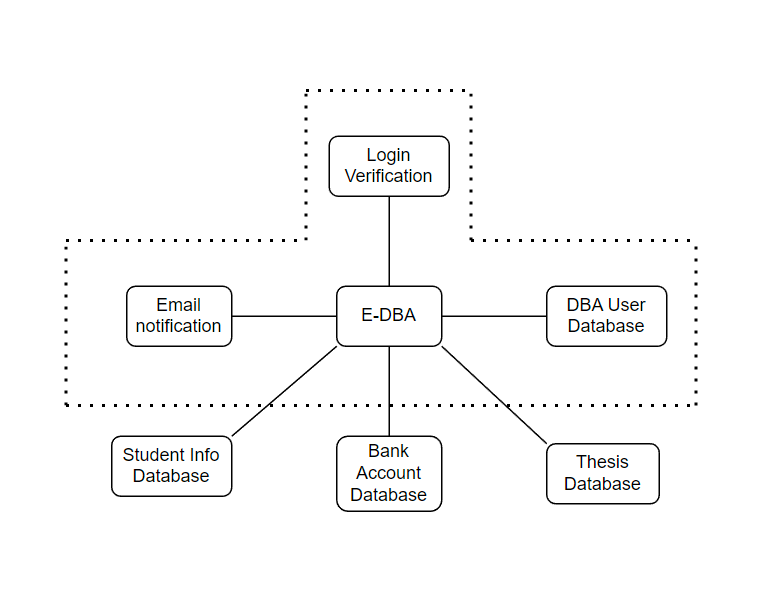
\includegraphics[width=0.75\linewidth]{picture/1241740968356.jpg}
    \caption{Product Perspective}
    \label{fig:enter-label}
\end{figure}

\section{Product Functions}
\FloatBarrier
\begin{figure}[H]
    \centering
    \begin{minipage}{0.42\linewidth}
        \centering
        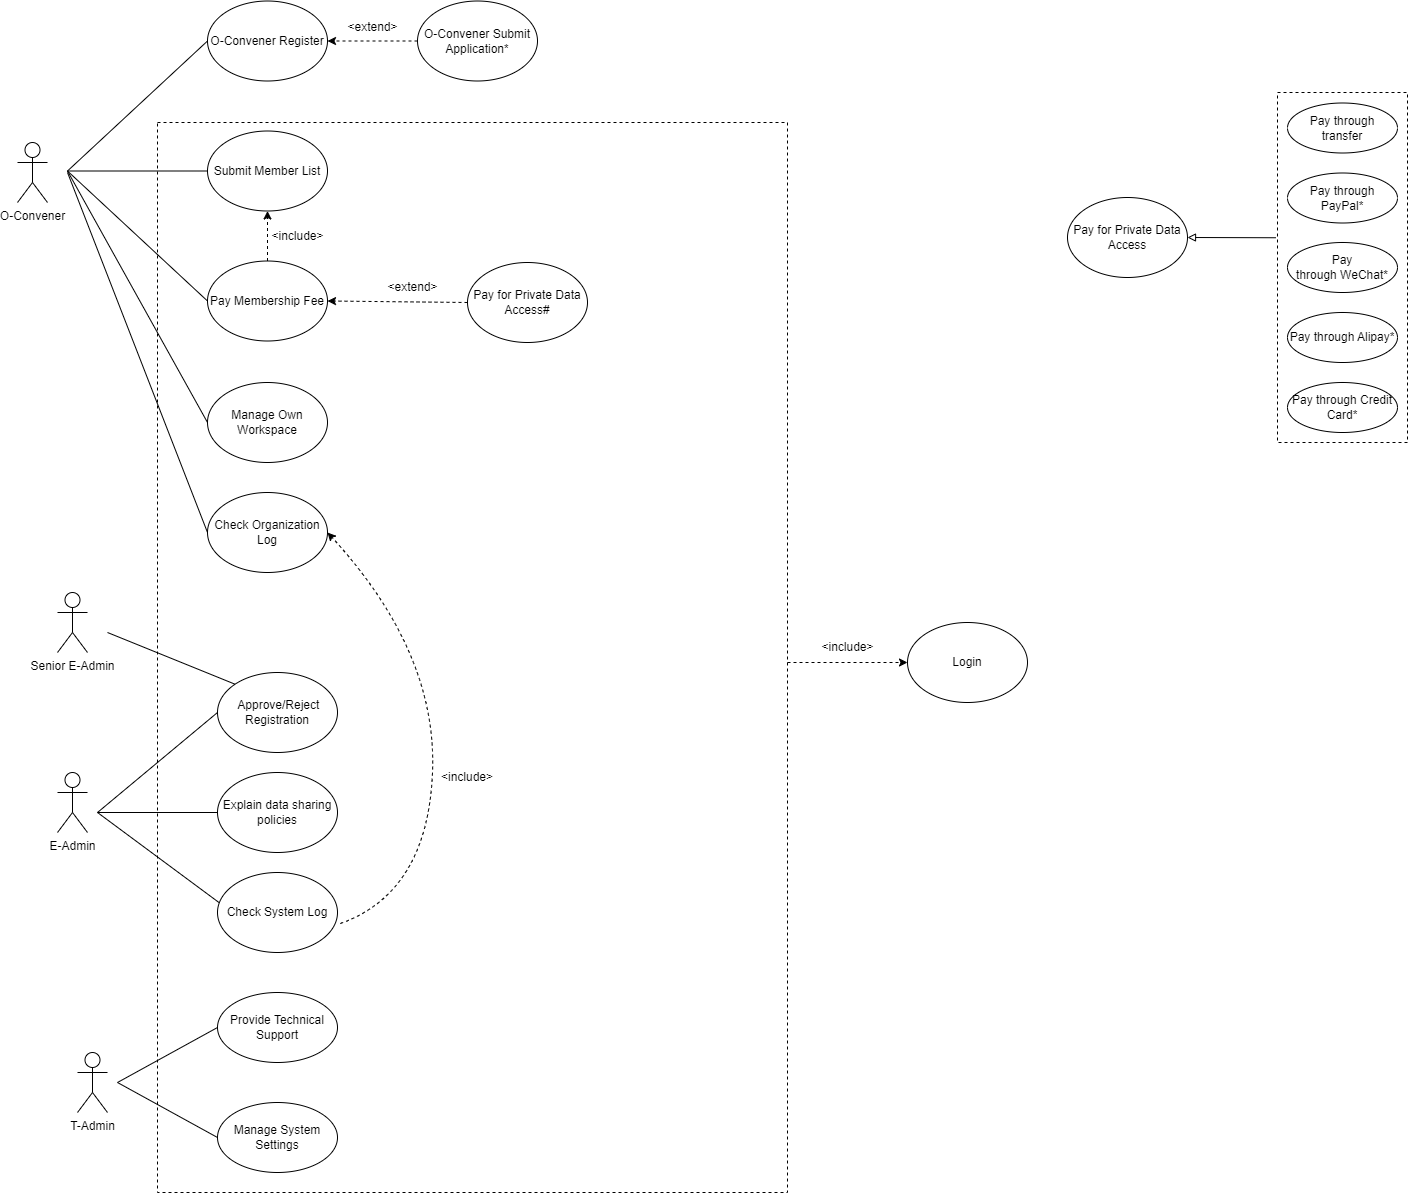
\includegraphics[width=\linewidth]{picture/WechatIMG190.jpg}
    \end{minipage}
    \hspace{0.04\linewidth} % 添加间隔
    \begin{minipage}{0.42\linewidth}
        \centering
        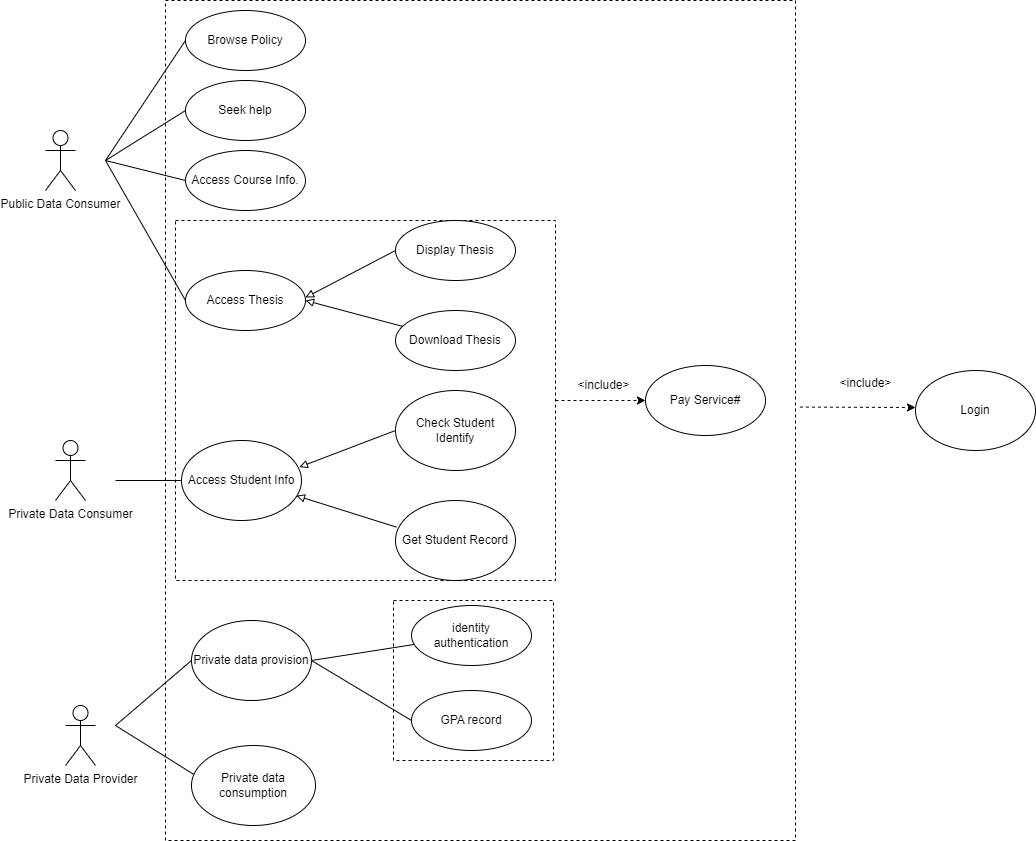
\includegraphics[width=\linewidth]{picture/WechatIMG191.jpg}
    \end{minipage}
    \caption{Product Function}
    \label{fig:product-function}
\end{figure}

\subsection{Basic Scenario}
The registration process initiates when the \textbf{O-Convener} completes the registration form (Step 1), providing contact information, institutional affiliation, and required documentation. Subsequently, the \textbf{E-Admin} or \textbf{Senior E-Admin} conducts a comprehensive review (Step 2), including material verification, authenticity validation, and background screening. Upon approval, system validation occurs (Step 3), generating a unique convener ID and activating service access privileges. Finalization (Step 4) triggers automated credential distribution and system onboarding initiation.

\subsection{Alternative Scenario}
\textbf{Registration Rejection:} In cases of administrative rejection, the system issues an automated notice detailing rejection rationale and appeal procedures, while preserving records for 30 days per GDPR compliance. \\
\textbf{Incomplete Submission:} System-level validation identifies missing elements through automated checks, flagging incomplete fields and initiating follow-up protocols requiring convener remediation before process continuation.

\section{User Classes and Characteristics}
\begin{itemize}
    \item \textbf{Admin}:
    \begin{itemize}
        \item \textbf{T-admin}: Responsible for overseeing and managing system functionality. Has access to the full suite of administrative controls.
        \item \textbf{E-admin}: Handles user and system management, including configuration of system features and settings.
        \item \textbf{Senior E-admin}: Manages both system and user configurations at an advanced level.
    \end{itemize}
    \textbf{Characteristics:} Must be responsive and make decisions to resolve user issues efficiently.
    
    \item \textbf{O-Convener}: Focuses on managing user lists, workspace organization, and service configurations for the system.  
    \textbf{Characteristics:} Must manage user access and configure services.

    \item \textbf{Data Provider and Data Consumer}:
    \begin{itemize}
        \item \textbf{Data Provider}: Supplies the system with data for processing and consumption.
        \item \textbf{Data Consumer}: Engages with the system to access and use provided data, including processing payments for data consumption.
    \end{itemize}
    \textbf{Characteristics:} Must be skilled in operating systems and data sorting.

    \item \textbf{End Users}: Individuals who interact with the system on a more basic level to access or utilize specific functionalities. End users are the primary consumers of the system's services, with access tailored to their specific needs.  
    \textbf{Characteristics:} Can basically use the system through instruction.
\end{itemize}

\section{Operating Environment}
We will use windows or linux as our poerating environment. We will also use database management system like MySQL to store our data


\section{Design and Implementation Constraints}
\begin{itemize}
    \item The system must adhere to a high level of security to protect sensitive data and user privacy.
    \item The system must be capable of connecting to and interacting with a database management system to store and retrieve data efficiently.
\end{itemize}

\section{User Documentation}
\begin{itemize}
    \item \textbf{User Manuals}: Comprehensive guides tailored to each user class (admin, end user, etc.), providing step-by-step instructions for system setup and usage.
    \item \textbf{On-line Help}: An integrated help system within the software that offers real-time support to solve user problems.
    \item \textbf{Tutorials}: Both video and text-based tutorials designed to help users understand how to operate the system effectively.
    \item \textbf{Release Notes}: A summary of updates and changes made in each version of the system to inform users of new features, fixes, or enhancements.
\end{itemize}

\section{Assumptions and Dependencies}

\textbf{Assumptions}:
\begin{itemize}
    \item The stability and reliability of third-party services integrated with the system.
\end{itemize}

\textbf{Dependencies}:
\begin{itemize}
    \item The project will rely on a database management system for development and data storage.
\end{itemize}

\chapter{System Features}

\section{Login}

\subsection{Description}
Login function for all users: T-admin, senior E-admin, E-admin, O-convener, Public Data provider, Private data consumer, Public Data consumer. The login page can be accessed from the main page of the software. Different types of users have different privileges. Medium priority.

\subsection{State diagrams / UI}
\begin{figure}[H]
    \centering
    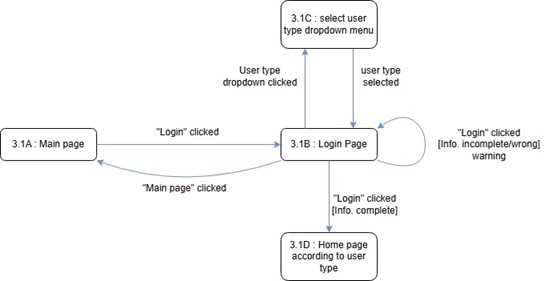
\includegraphics[width=0.75\linewidth]{picture/picture312.jpg}
    \caption{State Diagrams}
    \label{fig:enter-label}
\end{figure}

\textit{Note:} Please refer to document in 4.1 for UI diagrams.

\textbf{Scenario 1: Login Success}
\begin{itemize}
    \item Assume users are on the main page.
    \item Users click the login button on the main page.
    \item System displays the login page.
    \item Users select user type and enter credentials.
    \item Users click the login button.
    \item System directs users to the home page.
\end{itemize}

\textbf{Scenario 2: Login Fail}
\begin{itemize}
    \item Assume users are on the main page.
    \item Users click the login button on the main page.
    \item System displays the login page.
    \item Users select user type and enter credentials.
    \item Users click the login button.
    \item System displays a login fail message.
    \item System returns to the login page.
\end{itemize}

\subsection{Functional Requirements}

TBD

\section{O-Convener}

\subsection{Description}
O-convener is specific to the organization that provides the managment of users and access rights. The O-convener can manage their own private workspace, maintain and grant new users access permission from their organization to use the E-DBA and as well as check the organization log. The addition of users is done either through system UI or from Excel files for batch input. Medium priority

\subsection{State diagrams / UI}
\begin{figure}[H]
    \centering
    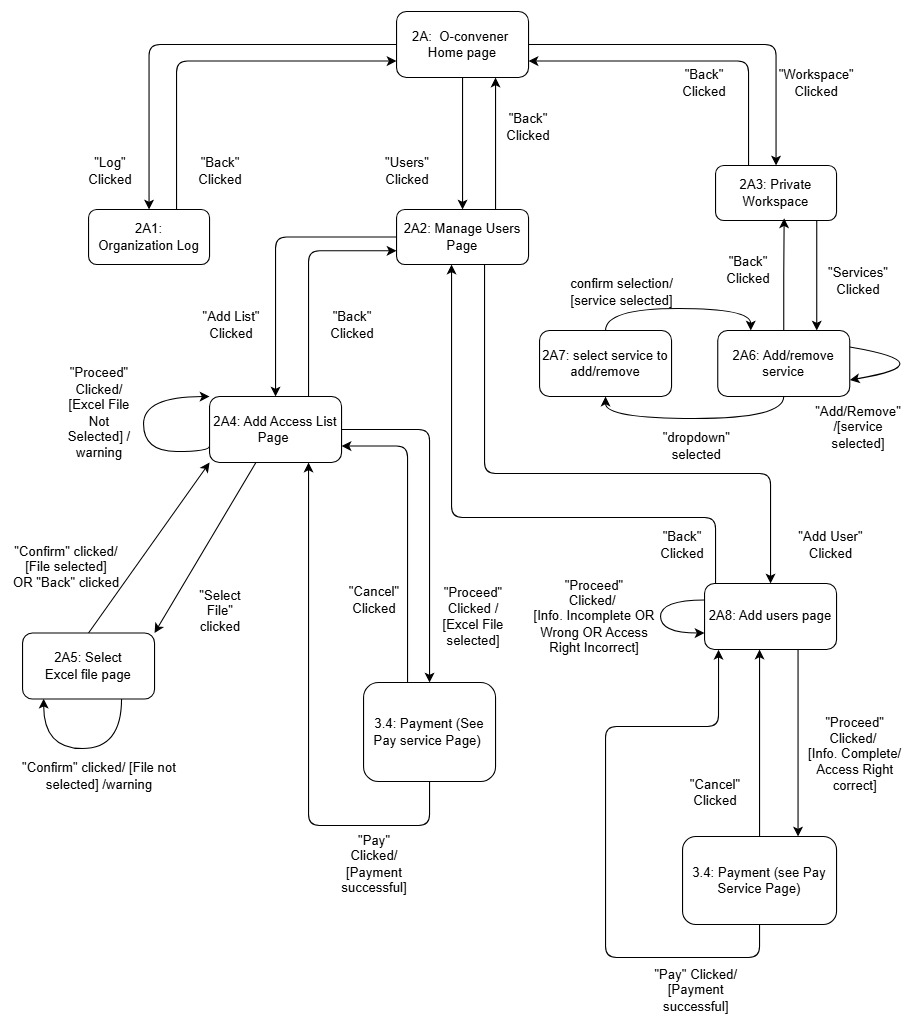
\includegraphics[width=0.75\linewidth]{picture/WechatIMG1905.jpg}
    \caption{State Diagrams}
    \label{fig:enter-label}
\end{figure}

\subsection*{Scenario 1: Manage Own Private Workspace}
\begin{itemize}
    \item From O-Convener home page.
    \item Enter Private Workspace.
\end{itemize}

\subsection*{Scenario 2: Manage Users – Add Users Through System UI}
\begin{itemize}
    \item From O-Convener home page.
    \item Enter Manage User page.
    \item Click "Add Users".
    \item Enter credentials and access rights.
    \item Save choice and proceed to payment.
    \item Finish and return to Manage User page.
\end{itemize}

\subsection*{Scenario 3: Manage Users – Add Users Through Excel Batch File}
\begin{itemize}
    \item From O-Convener home page.
    \item Enter Manage User page.
    \item Click "Add Access List".
    \item Input Excel file.
    \item Save choice and proceed to payment.
    \item Finish and return to Manage User page.
\end{itemize}

\subsection*{Scenario 4: Check Organization Log}
\begin{itemize}
    \item From O-Convener home page.
    \item Enter Check Log page.
    \item Return to Home page.
\end{itemize}

\section{E-Admin \& Senior E-Admin}

\subsection{Description}
In the system, E-Admin could check system log through inspecting the system log status of each user, while they could explain data sharing policy through write the explanation for selected data sharing policy. And they could also approve or reject application through checking the content of application and deciding whether approve the application or reject. However, Senior E-Admin could only approve or reject application. 

\subsection{Stimulus/Response Sequence}

\begin{figure}[H]
    \centering
    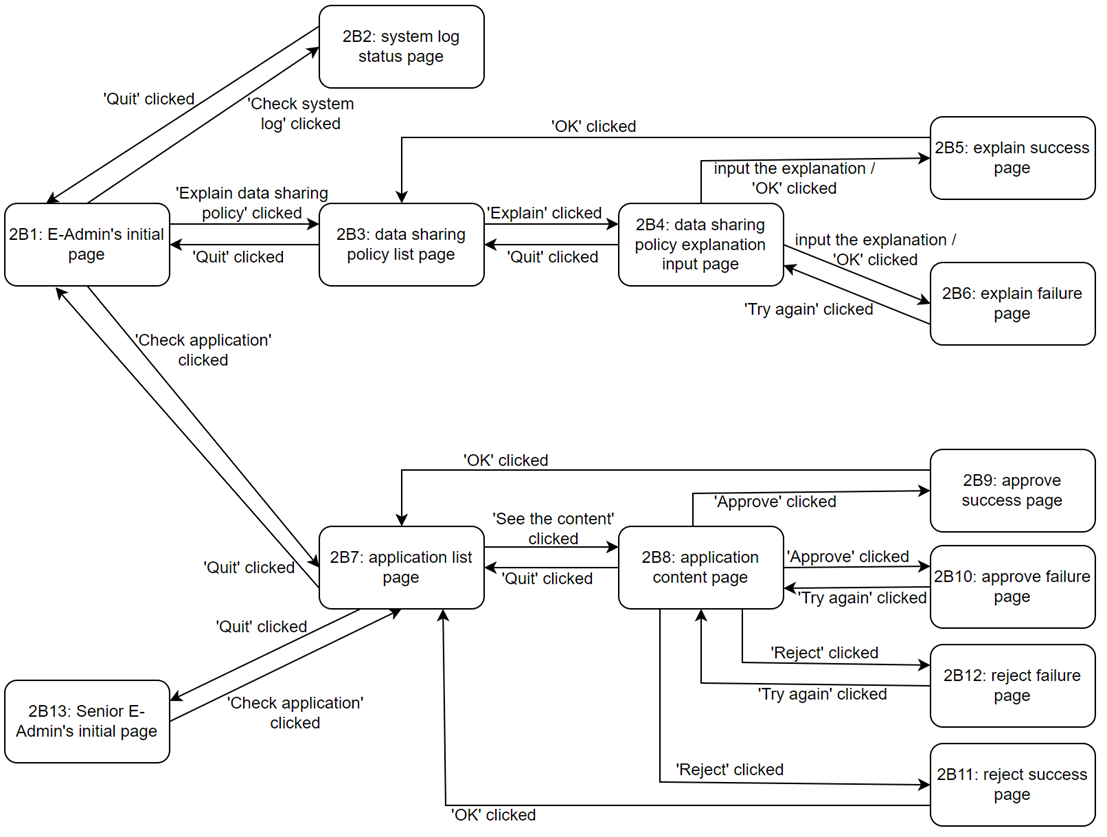
\includegraphics[width=0.75\linewidth]{picture/201391923.png}
    \caption{State Diagrams}
    \label{fig:enter-label}
\end{figure}

\textbf{Basic Scenario}
\begin{itemize}
    \item The E-Admin/Senior E-Admin logs in.
    \item The system displays the E-Admin’s/Senior E-Admin’s initial page.
    \item The E-Admin clicks ‘Check System Log’.
    \item The system displays the system log status page.
    \item The E-Admin clicks ‘Explain Data Sharing Policy’.
    \item The system displays the data sharing policy list page.
    \item The E-Admin clicks ‘Explain’.
    \item The system displays the data sharing policy explanation input page.
    \item The E-Admin inputs the explanation and clicks ‘OK’.
    \item The system displays the explanation success page if successful, otherwise, displays the explanation failure page.
    \item The E-Admin clicks ‘OK’ or ‘Try Again’.
    \item The system returns to the data sharing policy list page or the data sharing policy explanation input page.
    \item The E-Admin clicks ‘Quit’.
    \item The system returns to the E-Admin’s initial page.
    \item The Senior E-Admin/E-Admin clicks ‘Check Application’.
    \item The system displays the application list page.
    \item The Senior E-Admin/E-Admin clicks ‘See the Content’.
    \item The system displays the application content page.
    \item The Senior E-Admin/E-Admin clicks ‘Approve’ or ‘Reject’.
    \item The system displays the approve success page or reject success page if successful, otherwise, displays the approve failure page or reject failure page.
    \item The Senior E-Admin/E-Admin clicks ‘OK’ or ‘Try Again’.
    \item The system returns to the application list page or the application content page.
    \item The Senior E-Admin/E-Admin clicks ‘Quit’.
    \item The system returns to the E-Admin’s/Senior E-Admin’s initial page.
\end{itemize}

\section{T-Admin}

\subsection{Description}
The user navigates through the T-Admin system to manage E-Admin accounts, respond to help requests, and manage vault applications. Actions include editing and updating account information, answering help requests, and navigating back to previous menus.


\subsection{Stimulus/Response Sequence}
\begin{figure}[H]
    \centering
    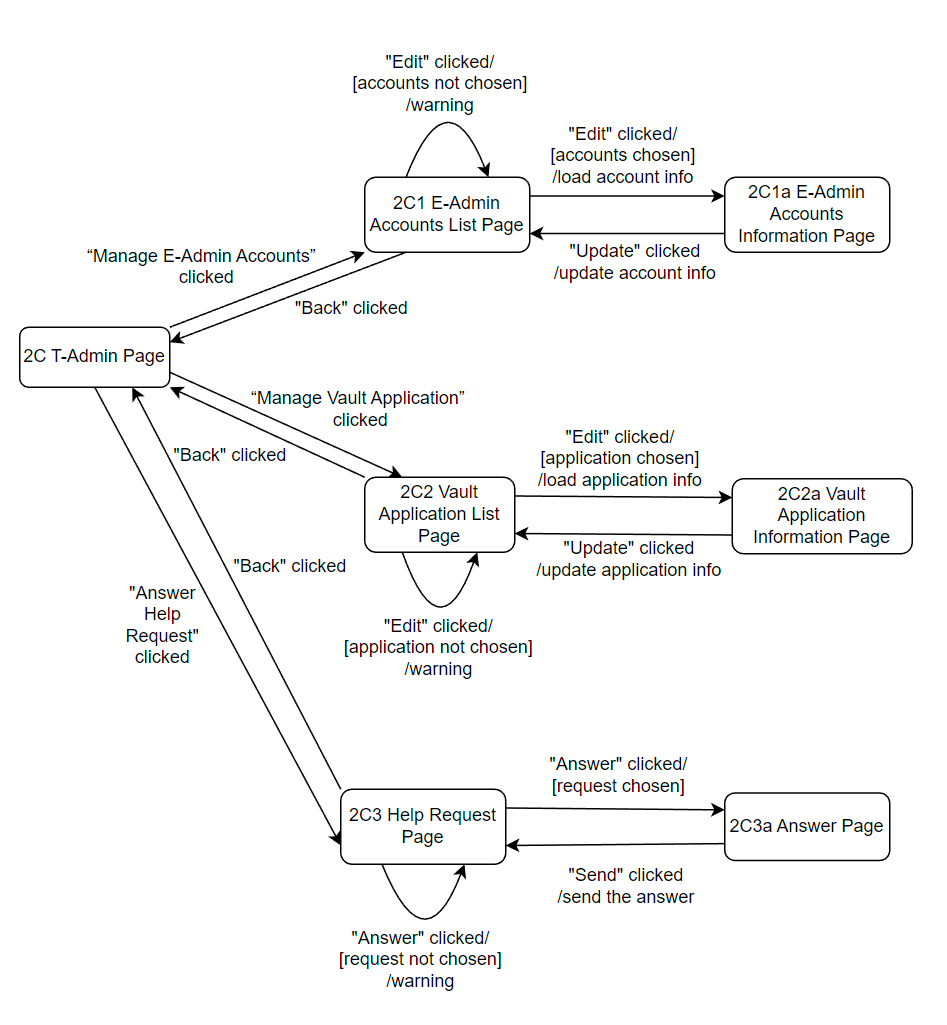
\includegraphics[width=0.75\linewidth]{picture/WechatIMG327.jpg}
    \caption{State Diagrams}
    \label{fig:enter-label}
\end{figure}

\begin{itemize}
    \item The user clicks “Manage E-Admin Accounts”. → The system displays the E-Admin accounts list.
    \item The user clicks “Edit”. → The system shows E-Admin account information.
    \item The user clicks “Update”. → The system goes back to the E-Admin accounts list page.
    \item The user clicks “Back”. → The system goes back to the manage page.
    
    \item The user clicks “Answer Help Request”. → The system shows the help request list.
    \item The user clicks “Answer”. → The system shows the answer page.
    \item The user clicks “Send”. → The system goes back to the help request list page.
    \item The user clicks “Back”. → The system goes back to the manage page.
    
    \item The user clicks “Manage Vault Application”. → The system displays the vault application list.
    \item The user clicks “Edit”. → The system shows vault application information.
    \item The user clicks “Update”. → The system goes back to the vault application list page.
    \item The user clicks “Back”. → The system goes back to the manage page.
    \item The user clicks “Back” again. → The system goes back to the T-Admin page.
\end{itemize}

\section{Public Data Consumer}

\subsection{Description}
The Public Data Consumer can browse policies, seek help, access course information, and access thesis. They can select policies to view details, submit help requests and check responses, choose courses to access information, and download theses after payment. The system provides success, failure, or warning feedback based on actions and allows navigation between pages.

\subsection{State diagrams / UI}
\begin{figure}[H]
    \centering
    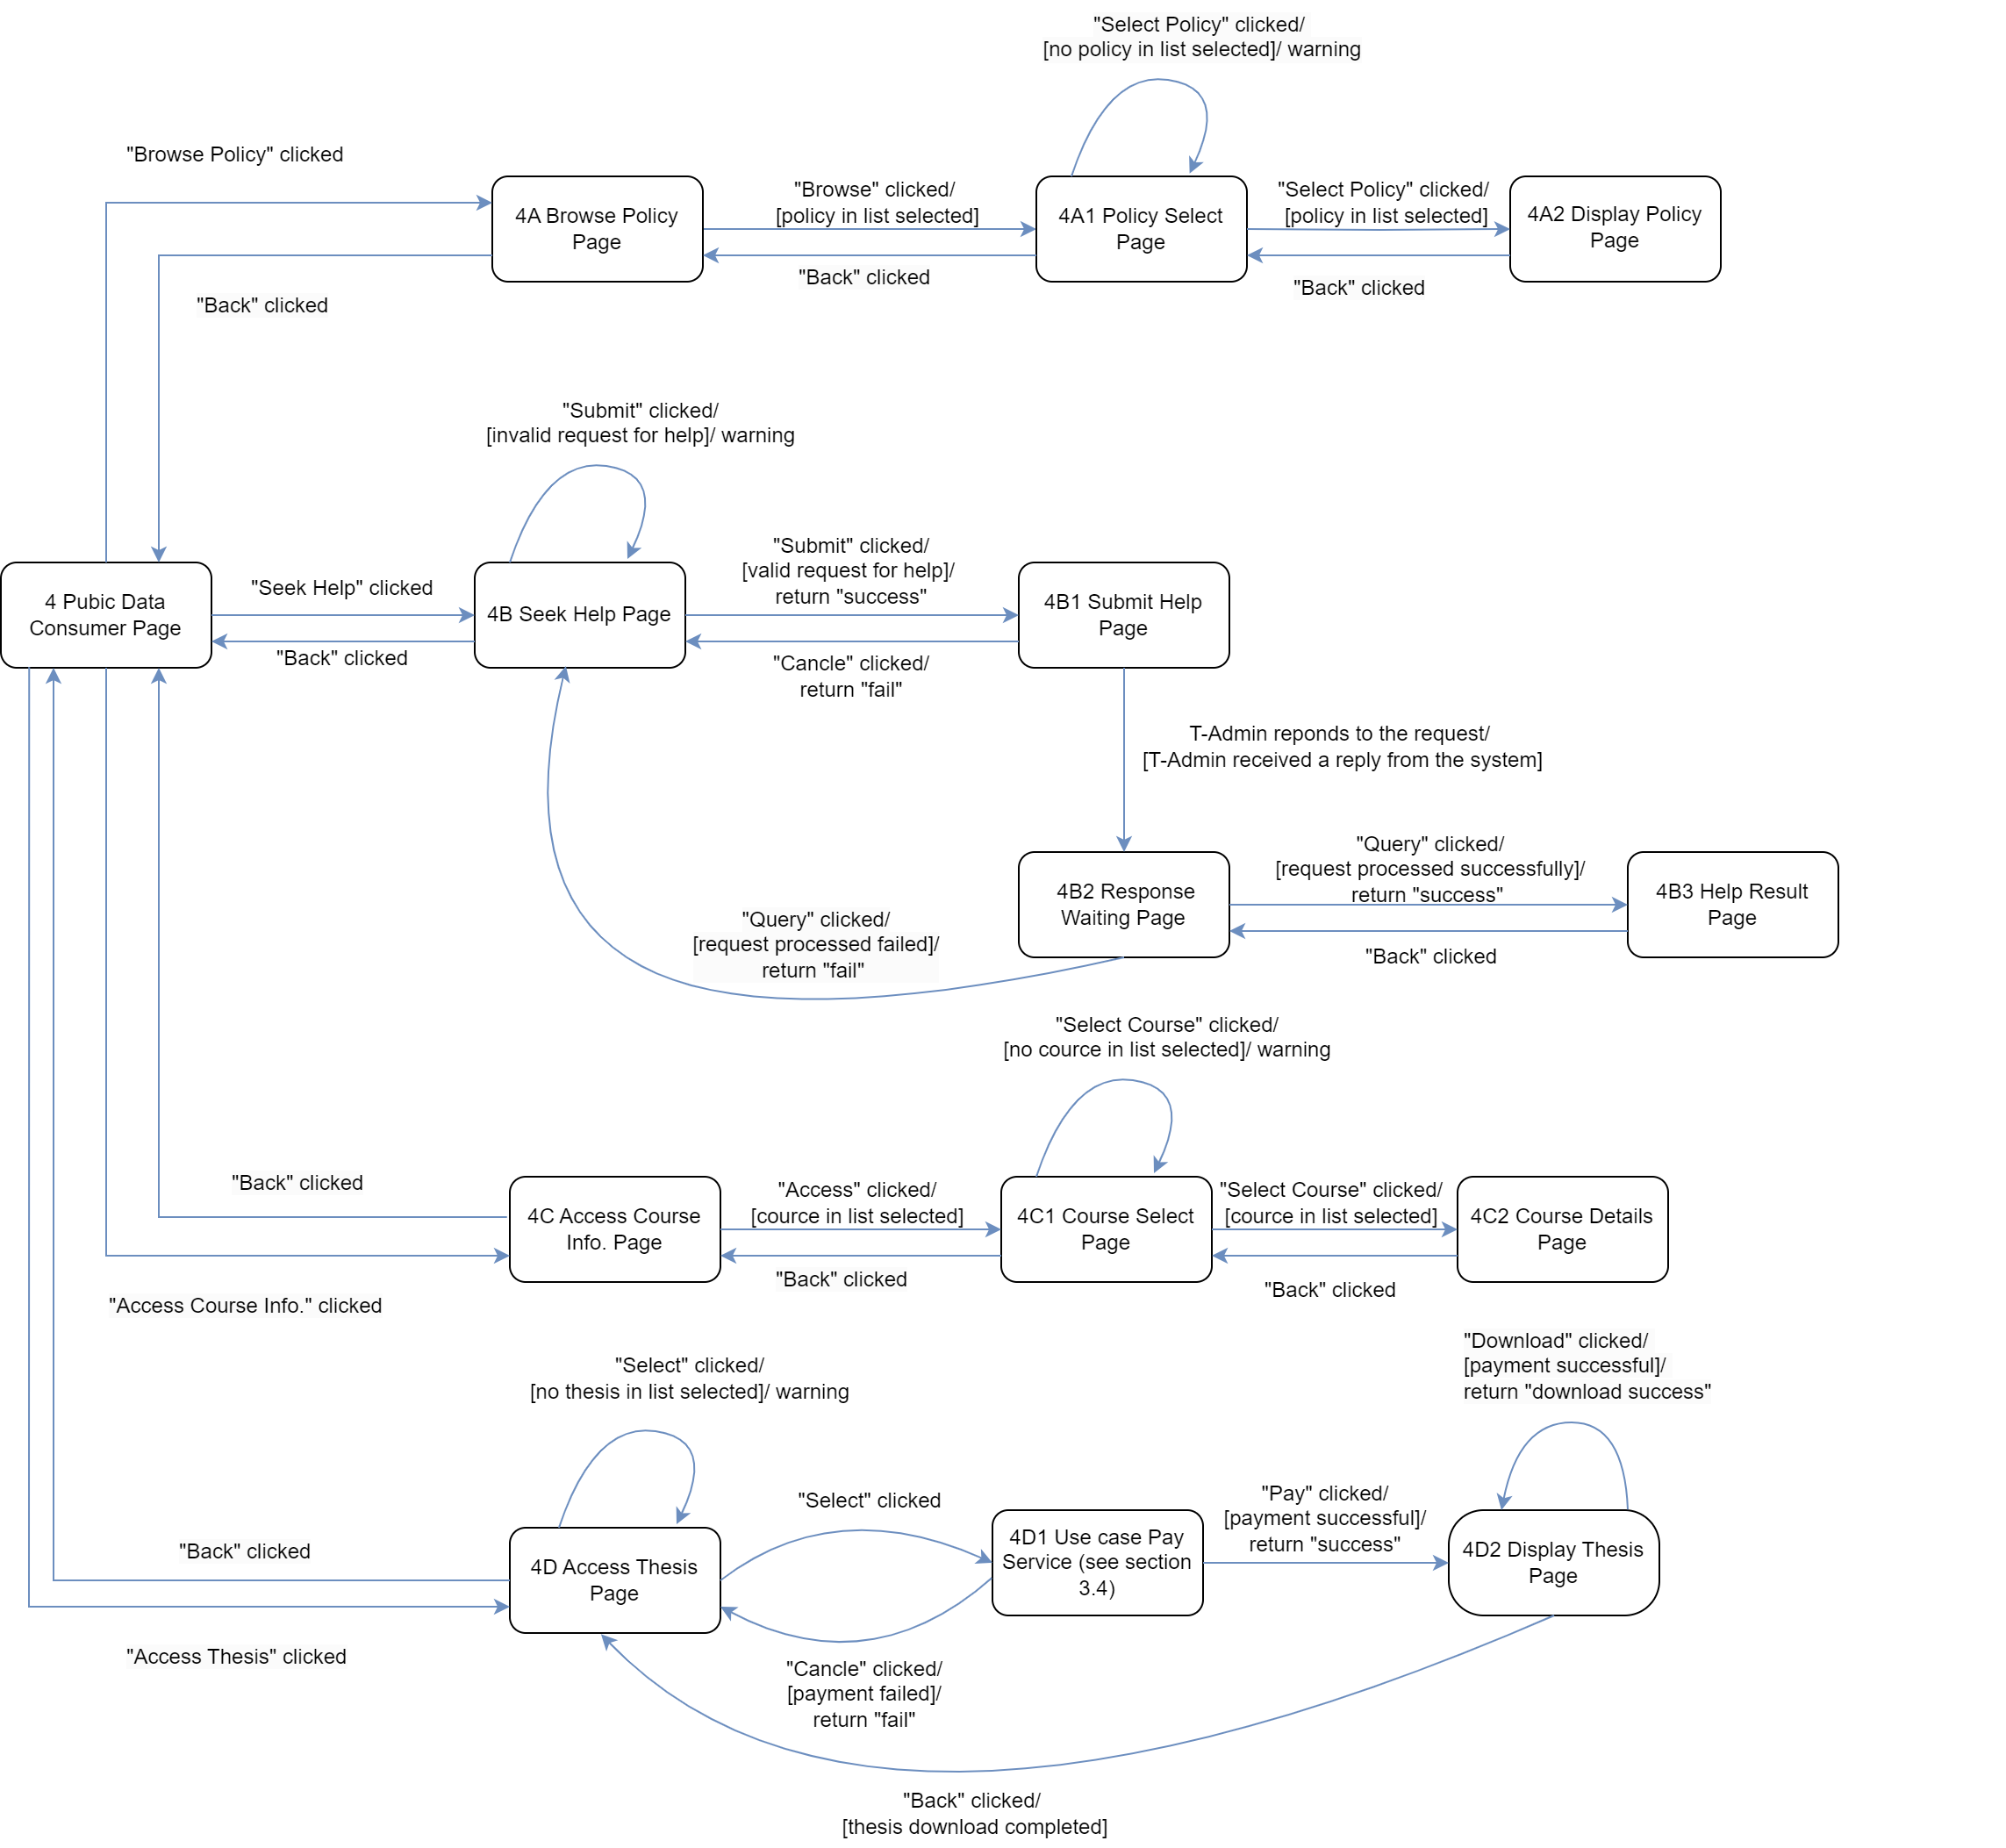
\includegraphics[width=0.75\linewidth]{picture/WechatIMG297.jpg}
    \caption{State Diagrams}
    \label{fig:enter-label}
\end{figure}

\textit{Note:} Please refer to document in 4.1 for UI diagrams.

\textbf{Basic Scenario}
\begin{itemize}
\item{Browse Policy}
    \begin{enumerate}
        \item User browses the policy list.
        \item Views policy details.
        \item Returns to the list at any time.
    \end{enumerate}

\item{Seek Help}
    \begin{enumerate}
        \item User submits a help request.
        \item Waits for T-Admin's reply.
        \item Ends the process after confirming the reply.
    \end{enumerate}

\item{Access Course Info}
    \begin{enumerate}
        \item User browses the course list.
        \item Views course details.
        \item Returns to the list at any time.
    \end{enumerate}

\item{Access Thesis}
    \begin{enumerate}
        \item Selects Thesis.
        \item Displays Thesis Content.
        \item Requests Download.
        \item Downloads Thesis.
    \end{enumerate}
\end{itemize}


\subsection{Functional Requirements}

TBD

\section{Pay Service}

\subsection{Description}
In the Pay Service use case, the actor could pay by PayPal, Credit Card, AliPay, WeChat or by money transfer through scan the QR code on the corresponding page, however, the system would initially only allow money transfer, and if the actor want to pay by other methods, he/she could go to the next page to select the payment method he/she want and pay the money.

\subsection{State diagrams / UI}
\begin{figure}[H]
    \centering
    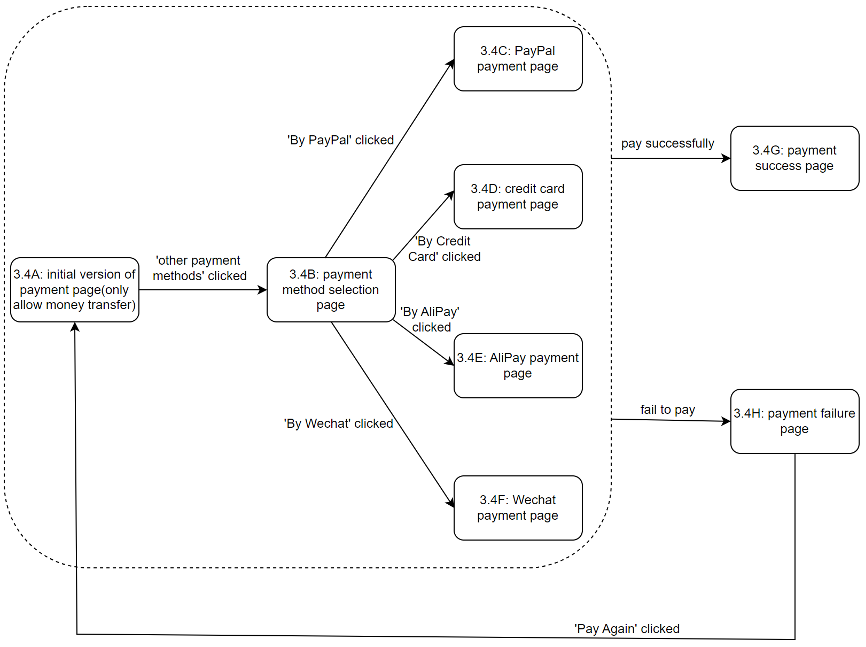
\includegraphics[width=0.75\linewidth]{picture/12312323.png}
    \caption{State Diagrams}
    \label{fig:enter-label}
\end{figure}

\textit{Note:} Please refer to document in 4.1 for UI diagrams.

\textbf{Basic Scenario} \\
The actor scan the QR code on the initial version of payment page and pay the money. \\
The system display the payment success page if the actor paid successfully, otherwise, the system display payment failure page
The actor click ‘other payment methods’ button. \\
The system display the payment method selection page. \\
The actor click ‘By PayPal’/’By Credit Card’/’By Alipay’/’By Wechat’ button.\\
The system display PayPal payment page/credit card payment page/AliPay payment page/Wechat payment page. \\
The actor scan the QR code on the PayPal payment page/credit card payment page/AliPay payment page/Wechat payment page and pay the money.\\
The system display the payment success page if the actor paid successfully, otherwise, the system display payment failure page.


\subsection{Functional Requirements}
TBD

\section{Data Provider}

\subsection{Description}
The data provider can add info to a new course or edit the info of an existing course. He can also set an interface for thesis sharing services by set corresponding links according to different services.

\subsection{Stimulus/Response Sequence}

\begin{figure}[H]
    \centering
    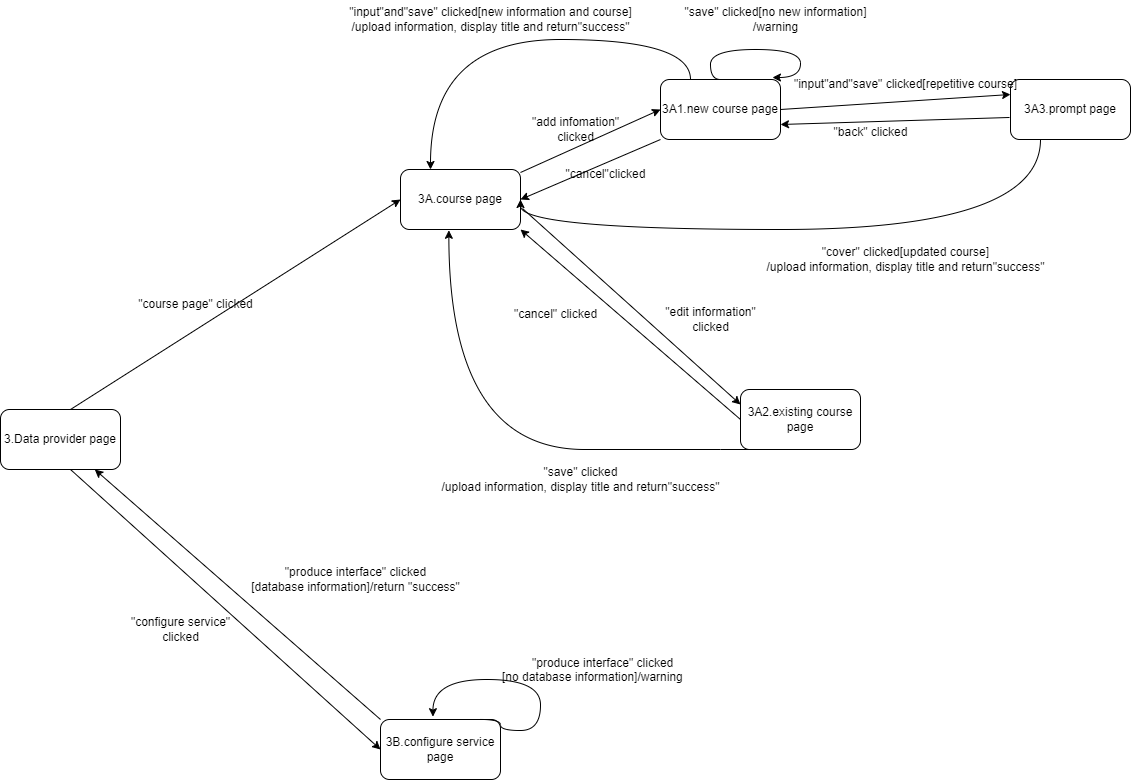
\includegraphics[width=0.75\linewidth]{picture/WechatIMG1904.jpg}
    \caption{State Diagrams}
    \label{fig:enter-label}
\end{figure}

\textbf{Basic Scenario}
\begin{itemize}
    \item The Private Data Provider clicks “add information/edit information”.
    \item The system displays the information page.
    \item The Private Data Provider adds/edits information.
    \item The system saves the information and displays it.
    \item The Private Data Provider then clicks “configure service”.
    \item The system displays the configure service page.
    \item The Private Data Provider adds a database and clicks “produce interface”.
    \item The system produces the interface.
\end{itemize}

\textbf{Alternative Scenario}

\begin{itemize}
    \item The Private Data Provider clicks “add information/edit information”.
    \item The system displays the information page.
    \item The Private Data Provider does not add new information or adds a repetitive course.
    \item If no new course is added, the system returns to the new course page.
    \item If a repetitive course is added, the system will go to the prompt page to check whether the author wants to overwrite the original course.
    \item The Private Data Provider then clicks “configure service”.
    \item The system displays the configure service page.
    \item The Private Data Provider does not add a database and clicks “produce interface”.
    \item The system gives a warning and returns to the configure service page.
\end{itemize}

\section{Private Data Consumer}

\subsection{Description}
The user accesses the system and navigates through various options to view and manage student information. The user can check student details, proceed to payment services (low priority), and return to previous menus as needed.

\subsection{Stimulus/Response Sequences}
\begin{figure}[H]
    \centering
    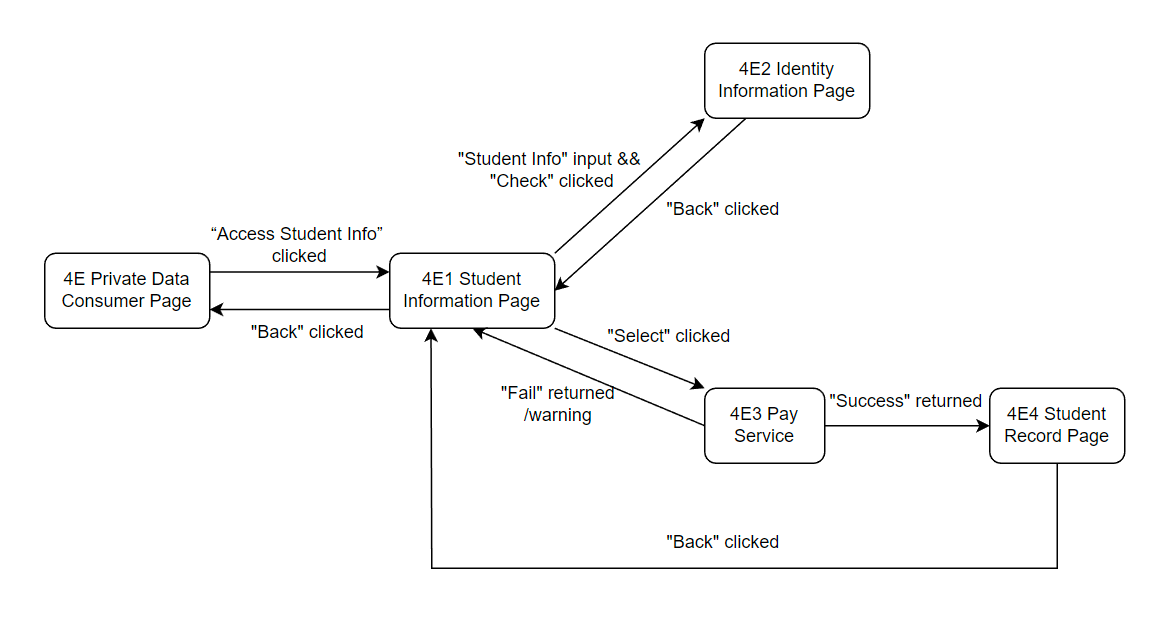
\includegraphics[width=0.75\linewidth]{picture/WechatIMG1901.jpg}
    \caption{State Diagrams}
    \label{fig:enter-label}
\end{figure}

\textbf{Basic Scenario}
\begin{itemize}
    \item The user clicks “Access Student Info”. → The system displays student information.
    \item The user inputs student info and clicks “Check”. → The system shows student identity information.
    \item The user clicks “Back”. → The system goes back to the student information page.
    \item The user clicks “Select”. → The system turns into the payment service.
    \item The user pays successfully. → The system shows the student record.
    \item The user clicks “Back”. → The system goes back to the information page.
    \item The user clicks “Back” again. → The system goes back to the private data consumer page.
\end{itemize}

\chapter{External Interface Requirements}

\section{User Interfaces}

\textbf{Please Visit the document User_Interface.pdf}

\section{Hardware Interfaces} 
TBD

\section{Software Interfaces} 
\begin{itemize}
    \item[1]Checking account validity and executing transfer processes through payment transfer methods (Transfer) (Paypal, WeChat, Alipay, Credit is TBD)
\end{itemize}

\section{Communications Interfaces}

\begin{itemize}
    \item[1]Email addresses and electronic forms, including proof documents required by the O-convener for registration.
    \item[2] Excel files required by a registered organization to authenticate student identity through batch input.
\end{itemize}

\chapter{Other Nonfunctional Requirements}

\section{Performance Requirements}
\begin{itemize}
    \item \textbf{Response Time}: To ensure a good user experience, the system should minimize delays, especially in critical operations such as real-time data access and identity verification.
    \item \textbf{Concurrency Handling}: During peak periods, such as the start of the school term or thesis submission deadlines, the system may experience a large number of concurrent users. The system must have strong concurrency handling capabilities to manage multiple user requests simultaneously.
    \item \textbf{Scalability}: The system should be scalable to accommodate future growth. New features should be easily added, and more users should be supported without affecting existing functionalities.
    \item \textbf{Data Consistency and Reliability}: For key operations such as payments and identity verification, data loss or inconsistencies must be prevented to avoid serious consequences. The system should have robust transaction management and error recovery mechanisms.
    \item \textbf{Resource Consumption}: Developers should optimize the code and architecture to ensure efficient use of resources, avoiding excessive consumption of server resources during operation.
\end{itemize}

\section{Safety Requirements}
\begin{itemize}
    \item \textbf{Data Breach Risk}: The system must prevent privacy violations and identity theft by encrypting data transmission and implementing strict access control mechanisms. Unauthorized access must be prohibited, and all user activities should be monitored.
    \item \textbf{Payment Security Risk}: The system should mitigate financial transaction risks by using multi-factor authentication and adopting certified secure payment gateways, ensuring the safety and reliability of payment channels.
    \item \textbf{System Stability Risk}: To prevent service interruptions, data loss, or corruption due to system instability, important data must be backed up regularly, and performance metrics should be continuously monitored.
\end{itemize}

\section{Security Requirements}
\begin{itemize}
    \item \textbf{Data Sharing Security}: The system must ensure that data is shared securely and transparently between different organizations. Data transmission must be encrypted, and only authorized parties should be able to access specific data.
    \item \textbf{Online Payment Security}: All payment operations must be secure to prevent financial fraud. Strict security measures must be taken to protect users' payment information, especially when handling personal financial details.
    \item \textbf{Non-tamperable Log Records}: System logs should be automatically categorized based on user activity and be non-modifiable to ensure the integrity of log data.
\end{itemize}

\section{Software Quality Attributes}
\subsection{For Users}
\begin{itemize}
    \item \textbf{Usability}: The system's user interface should be easy to use for individuals in different roles, with detailed guidance to help them get started quickly.
    \item \textbf{Reliability}: The system should run stably, minimizing the risk of failures and ensuring a quick recovery if issues arise.
    \item \textbf{Efficiency}: The system should respond quickly to user actions, whether browsing public information or querying private data.
\end{itemize}

\subsection{For Developers}
\begin{itemize}
    \item \textbf{Maintainability}: Code structure should be clear, following best practices, to ensure easier updates and iterations.
    \item \textbf{Compatibility}: The system should function correctly across various operating systems and browsers.
    \item \textbf{Flexibility}: The system should have flexible service interfaces for easy integration with external systems and support customizable configurations based on organizational needs.
    \item \textbf{Testability}: A comprehensive testing framework should be established, covering unit tests, integration tests, stress tests, and others.
    \item \textbf{Compliance}: The system should adhere to relevant laws and regulations, particularly those relating to personal data protection, following strict privacy guidelines.
\end{itemize}

\section{Business Rules}
\begin{itemize}
    \item \textbf{Roles and Permissions}: Different users and organizations have specific access rights and permissions. Only authorized users can perform critical operations like identity verification and payment processing.
    \item \textbf{Data Privacy}: The system must ensure that sensitive personal information is protected according to privacy regulations, restricting access to authorized personnel only.
\end{itemize}



\chapter{Other Requirements}

\section{Appendix A: Glossary}
\begin{itemize}
    \item \textbf{Reliability}: The ability of the database software to perform its required functions under stated conditions for a specified period of time without failure.
    
    \item \textbf{Efficiency}: The ability of the database software to perform tasks quickly and with minimal resource consumption.
    
    \item \textbf{Scalability}: The ability of the database software to handle increasing amounts of data and users.
    
    \item \textbf{Maintainability}: The ability of the database software to be modified, updated, or repaired over time.
    
    \item \textbf{Compatibility}: The ability of the database software to work the same as other systems, platforms, or tools.
    
    \item \textbf{Flexibility}: The ability of the database software to adapt to changing requirements or environments.
    
    \item \textbf{Testability}: The ability of the database software to be tested to ensure it meets functional and non-functional requirements.
\end{itemize}

\section{Appendix B: Analysis Models}
\subsection{Class Diagrams}
\begin{figure}[H]
    \centering
    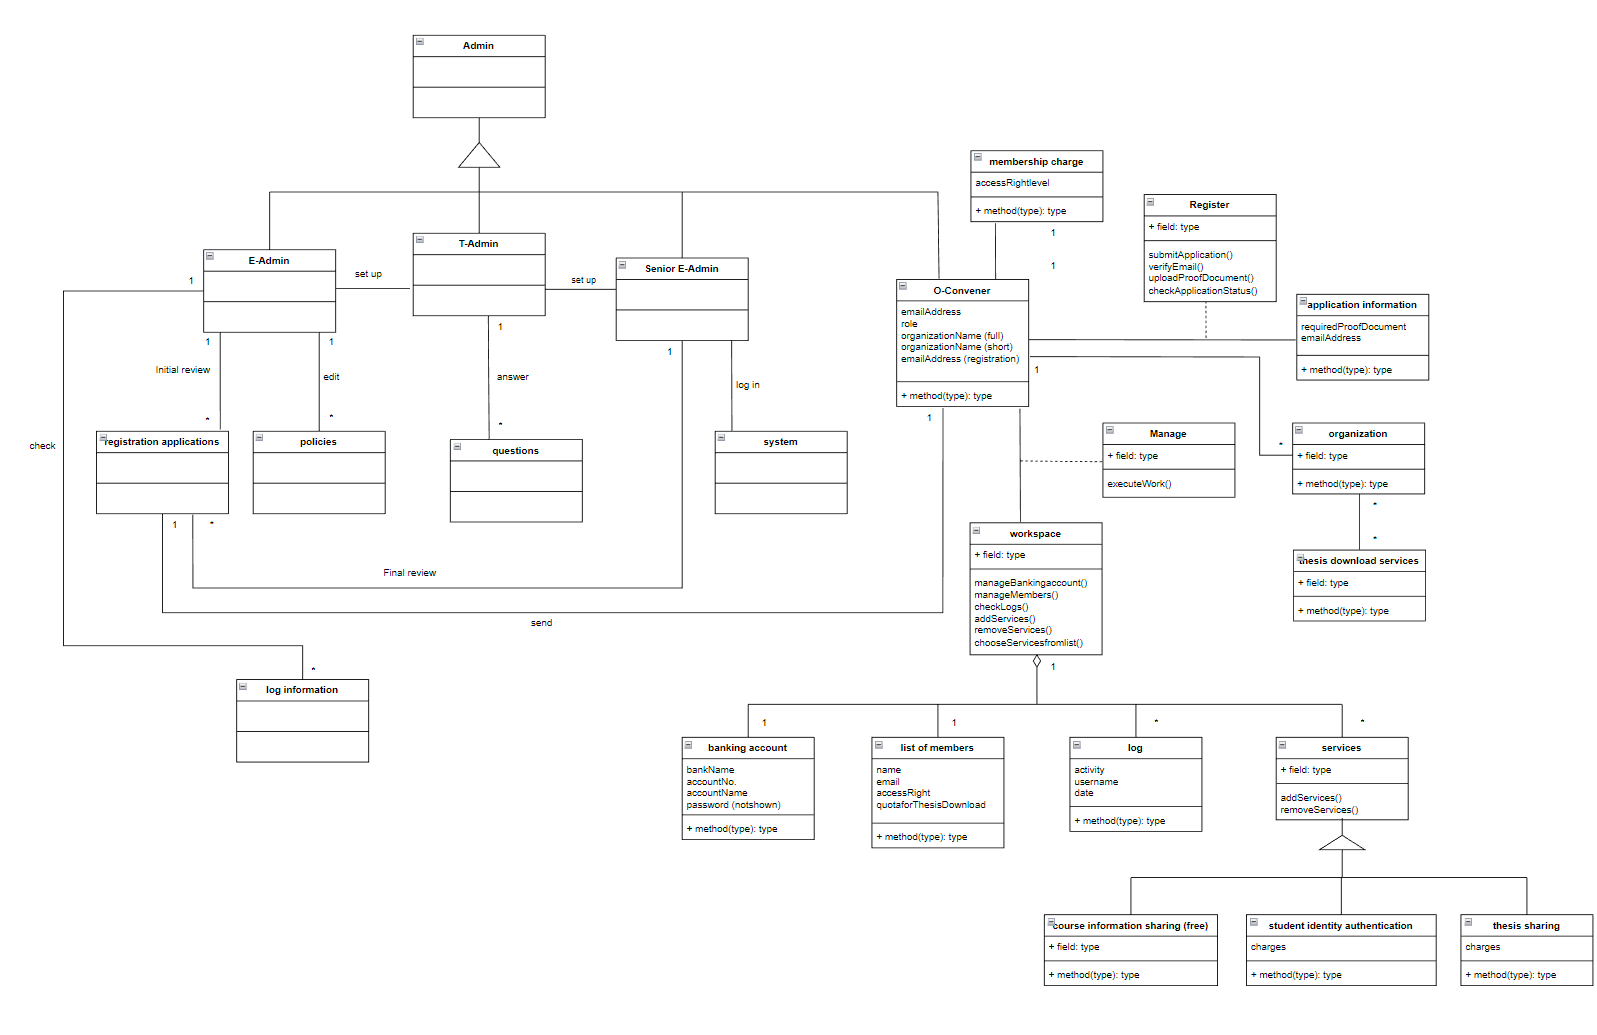
\includegraphics[width=0.75\linewidth]{picture/20250318214541.png}
    \caption{Class Diagrams}
    \label{fig:enter-label}
\end{figure}

\begin{figure}[H]
    \centering
    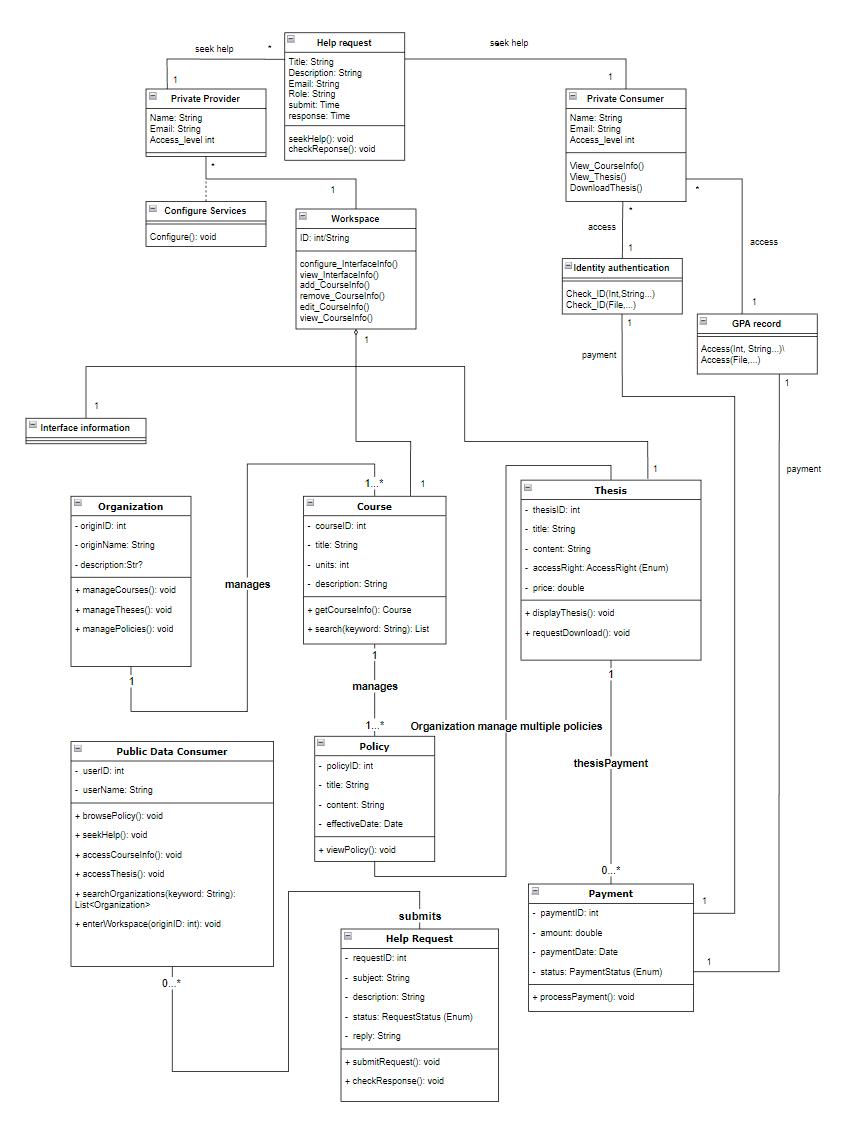
\includegraphics[width=0.75\linewidth]{picture/20250318214546.png}
    \caption{Class Diagrams}
    \label{fig:enter-label}
\end{figure}

\subsection{Sequence Diagrams}
\begin{figure}[H]
    \centering
    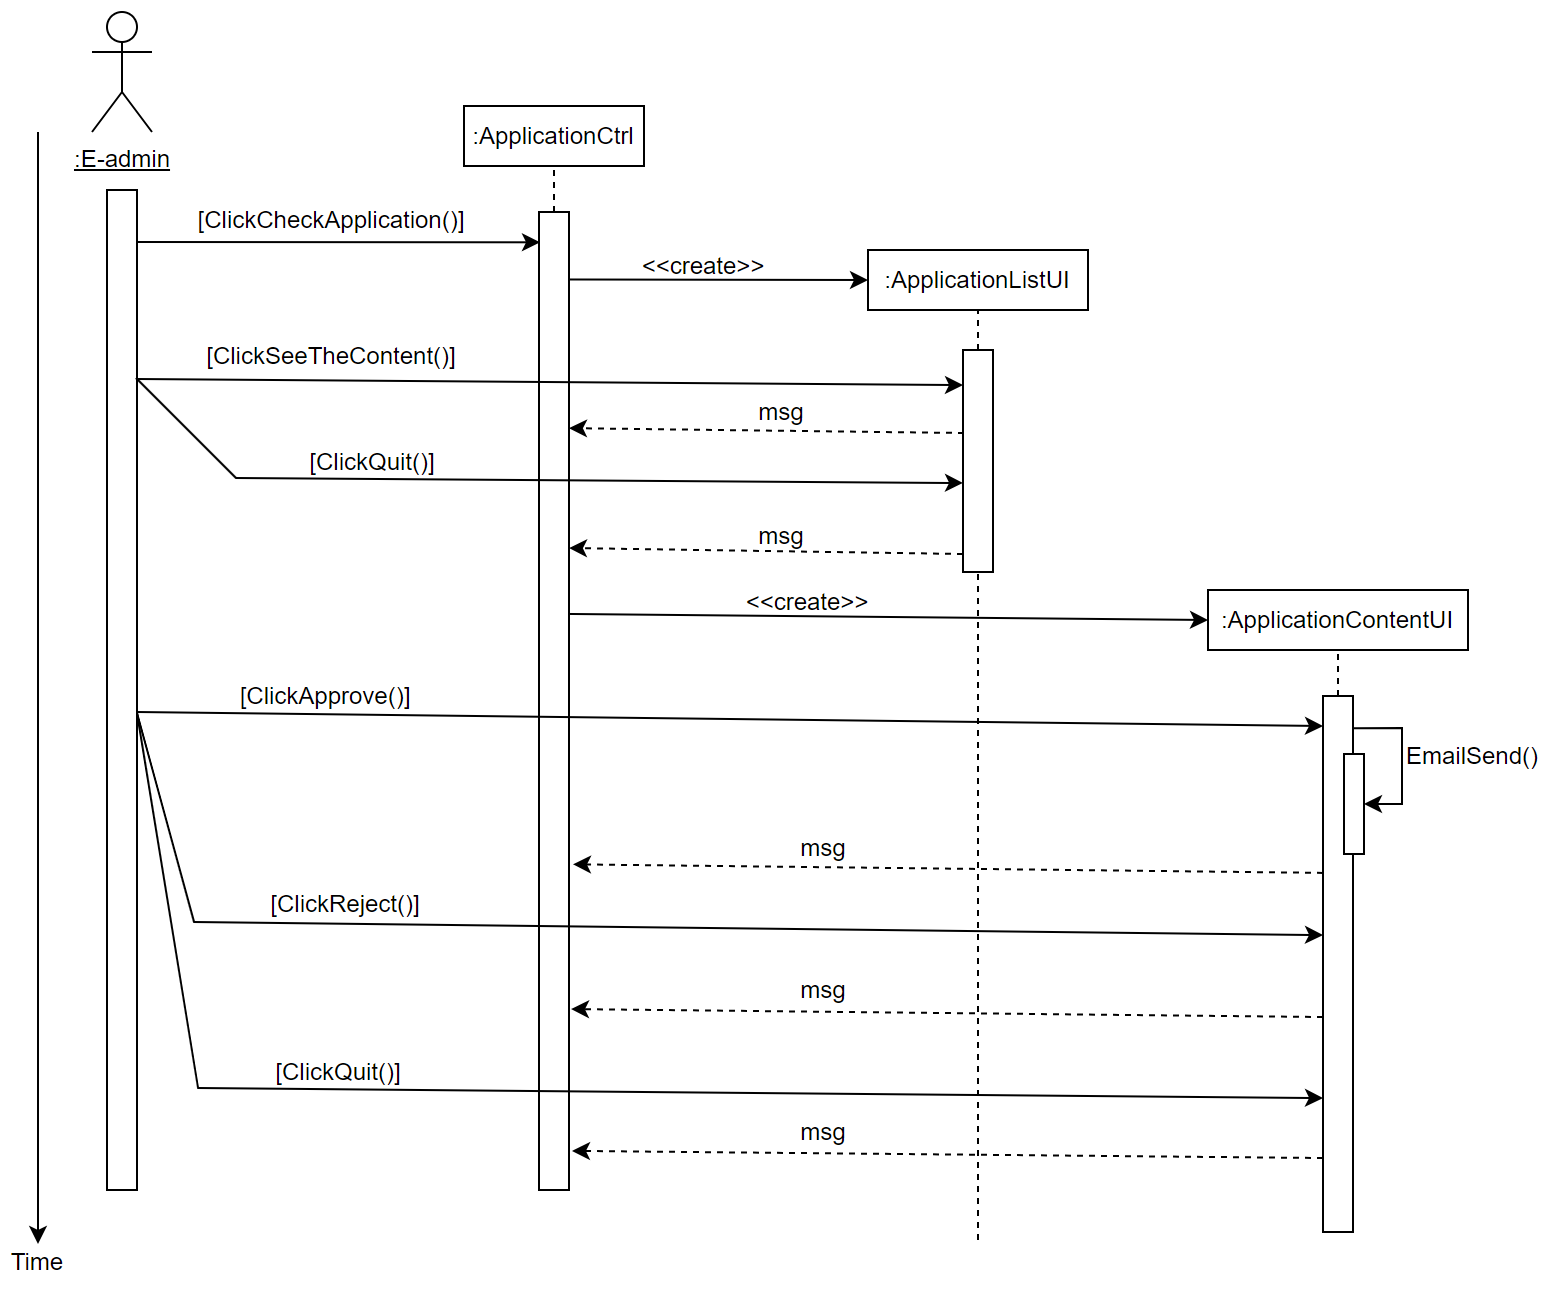
\includegraphics[width=0.75\linewidth]{picture/WechatIMG551.jpg}
    \caption{Sequence Diagrams}
    \label{fig:enter-label}
\end{figure}

\section{Appendix C: Issues List}
\begin{itemize}
    \item 4.2 TBD
    \item 6.2 TBD
\end{itemize}

% \chapter{Temporary}

% If there are any changes to the teacher's requirements, these will be copied to where they should be.
 
\nocite{*}
\printbibliography[heading=bibintoc]

\end{document}